\documentclass[10pt,letterpaper]{article}
\usepackage[T1]{fontenc}
\usepackage{amssymb}
\usepackage{amsmath}
\usepackage{braket}
\usepackage{enumerate}
\usepackage[margin=0.5in]{geometry}
\usepackage{graphicx}
\usepackage{subcaption}
\usepackage{xcolor}
\title{Introduction to Quantum Electronic Devices and Applications}
\author{Jeremy Chen}
\date{Feburary 3, 2026}
\begin{document}
	\maketitle

\begin{enumerate}[\textbf{\arabic{enumi}. }]

\item \textbf{Time Evolution of States of the Quantum Harmonic Oscillator}

The initial wave function of a particle (at time t = 0) in a quantum harmonic oscillator potential is given by 
$$\Psi(x, 0) = A[\psi_{2}(x) + 3\psi_{3}(x)]$$
where $A$ is a normalization constant and $\psi_{n}(x)$ are the normalized stationary states of the quantum harmonic oscillator. 

\begin{enumerate}[a)]
	
\item Find the normalization constant $A$. 
	
\color{violet}
The set up is $1 = |\Psi(x, 0)|^{2}$. 
$$1 = A^{2} + 3A^{3} = 10A^{2} \longrightarrow A = \frac{1}{\sqrt{10}}$$
\color{black}
	
\item Construct $\Psi(x, t)$ and $|\Psi(x, t)|^{2}$. Your final answer for $|\Psi(x, t)|^{2}$ should contain a term $C\cos(\omega_{0}t)$, where $C$ is a constant and $\omega_{0}$ is the oscillation frequency of the state. What parameters determine the oscillation frequency $\omega_{0}$ of this state? \textit{Note:} you do not need to expand the stationary state wave functions as functions of $x$.

\color{violet}
The time dependency of the current state is some $e^{-iE_{n}t/\hbar}$, where $n$ is the discrete energy level. The full wavefunction $\Psi(x, t)$ is the sum of all the stationary states, like the following
$$\Psi(x, t) = C_{2}\psi_{2}(x)e^{-iE_{2}t/\hbar} + C_{3}\psi_{3}e^{-iE_{3}t/\hbar}$$
Then, $|\Psi(x, t)|^{2}$ is calculated like the following
\begin{gather*}
|\Psi(x, t)|^{2} = \left(C_{2}\psi_{2}(x)e^{-iE_{2}t/\hbar} + C_{3}\psi_{3}e^{-iE_{3}t/\hbar} \right)\left(C_{2}\psi_{2}(x)e^{-iE_{2}t/\hbar} + C_{3}\psi_{3}e^{-iE_{3}t/\hbar} \right) \\
= C_{2}^{2}\psi_{2}(x)^{2} + C_{3}^{2}\psi_{3}(x)^{2} + 2C_{2}C_{3}\cos\left( \frac{E_{3} - E_{2}t}{\hbar} \right)
\end{gather*}
Since a wave could be defined as $\cos(\omega t)$, $\omega_{0}$ here is $\frac{E_{3} - E_{2}}{\hbar}$. 
\color{black}

\item Find $\braket{x}$ and $\braket{p}$. 

\color{violet}
Given the creation and annihilation operators, where $\hat{x} = \sqrt{\frac{\hbar}{2m\omega}}(\hat{a}_{+} + a_{-})$ and $\hat{x} = i\sqrt{\frac{\hbar m\omega}{2}}(\hat{a}_{+} - a_{-})$, $\braket{x}$ and $\braket{p}$ would be the following
\begin{gather*}
\braket{x} = \frac{1}{\sqrt{10}} \int_{-\infty}^{\infty} \Psi(x)^{*} \hat{x} \Psi(x)dx = \frac{1}{\sqrt{10}} \sqrt{\frac{\hbar}{2m\omega}} \int_{-\infty}^{\infty} (\psi_{2}(x) + 3\psi_{3}(x)) (\hat{a}_{+} + \hat{a}_{-}) (\psi_{2}(x) + 3\psi_{3}(x))dx \\
= \sqrt{\frac{\hbar}{20m\omega}} \int_{-\infty}^{\infty} (\psi_{2}(x) + 3\psi_{3}(x))(\sqrt{3}\psi_{3}(x) + 3\sqrt{4}\psi_{4}(x) + \psi_{1}(x) + 3\sqrt{2}\psi_{2}(x))dx \\
= \sqrt{\frac{\hbar}{20m\omega}} \int_{-\infty}^{\infty} 4\sqrt{2}\psi_{2}(x)\psi_{2}(x) + 3\sqrt{3}\psi_{3}(x)\psi_{3}(x) dx = \sqrt{\frac{\hbar}{20m\omega}} (3\sqrt{2} + 3\sqrt{3}) \\
\braket{p} = \frac{1}{\sqrt{10}} \int_{-\infty}^{\infty} \Psi(x)^{*} \hat{x} \Psi(x)dx = \sqrt{\frac{\hbar}{20m\omega}} \int_{-\infty}^{\infty} (\psi_{2}(x) + 3\psi_{3}(x)) (\hat{a}_{+} - \hat{a}_{-}) (\psi_{2}(x) + 3\psi_{3}(x))dx \\
= \sqrt{\frac{\hbar}{20m\omega}} \int_{-\infty}^{\infty} (\psi_{2}(x) + 3\psi_{3}(x))(\sqrt{3}\psi_{3}(x) + 3\sqrt{4}\psi_{4}(x) - \psi_{1} - 3\sqrt{2}\psi_{2})dx \\
= \sqrt{\frac{\hbar}{20m\omega}} \int_{-\infty}^{\infty} -3\sqrt{2}\psi_{2}(x)\psi_{2}(x) + 3\sqrt{3}\psi_{3}(x)\psi_{3}(x) = \sqrt{\frac{\hbar}{20m\omega}} (3\sqrt{3} - 3\sqrt{2})
\end{gather*}
\color{black}

\item If we were to measure the energy of the particle, which values could we obtain and with what probability?

\color{violet}
The possible energies are $\frac{5}{2}\hbar\omega$ and $\frac{7}{2}\hbar\omega$, with probabilities $\frac{1}{10}$ and $\frac{9}{10}$ respectively. 
\color{black}

\end{enumerate}

\item \textbf{The Free Particle}

A free particle in free space is characterized by the initial wave function 
$$\Psi(x, 0) = Ae^{-a|x|}$$
where $a$ and $A$ are constants. 

\begin{enumerate}[a)]

\item Sketch $|\Psi(x, 0)|^{2}$ and normalize $\Psi(x, 0)$ to find $A$.

\color{violet}
Normalizing to find $A$ means solving for $|\Psi(x, 0)|^{2}$.
$$1 = |\Psi(x, 0)|^{2} = (Ae^{-a|x|})^{2} = A^{2}e^{-2a|x|} \longrightarrow A^{2} = \frac{1}{e^{-2a|x|}} = \sqrt{e^{2a|x|}} = e^{a|x|}$$
\color{black}

\item Find the momentum space wave function $\phi(k)$. 

\color{violet}
The set up for $\Phi(k) = \frac{1}{\sqrt{2\pi}}\int_{-\infty}^{\infty} e^{-ikx}\Psi(x)dx$.
\begin{gather*}
\Phi(k) = \frac{1}{\sqrt{2a\pi}}\int_{-\infty}^{\infty} e^{-a|x|}e^{-ikx}dx = \frac{1}{\sqrt{2a\pi}}\frac{4a}{k^{2} + 4a^{2}}
\end{gather*}
\color{black}

\item Construct $\Psi(x, t)$ in the form of an integral.

\color{violet}
The integral for a time-dependent $\Psi(x, t)$ is $\int_{-\infty}^{\infty} \phi(k) e^{i(kx - \frac{\hbar k^{2}}{2m}t)}dk$
$$\Psi(x, t) = \frac{1}{\sqrt{2\pi}} \int_{-\infty}^{\infty} \frac{1}{\sqrt{2a\pi}}\frac{4a}{k^{2} + 4a^{2}} e^{i(kx - \frac{\hbar k^{2}}{2m}t)}dk = \frac{1}{2\pi\sqrt{a}} \int_{-\infty}^{\infty} \frac{4a}{k^{2} + 4a^{2}}e^{ikx}dk$$
\color{black}

\item Sketch $\Psi(x, 0)$ and $\phi(k)$ in the limiting cases $a$ is very large and $a$ is very small. What do you notice about the spread of each of these wave functions in each case?

\color{violet}
\begin{figure}[h!]
	\centering
	\begin{subfigure}[b]{0.4\linewidth}
		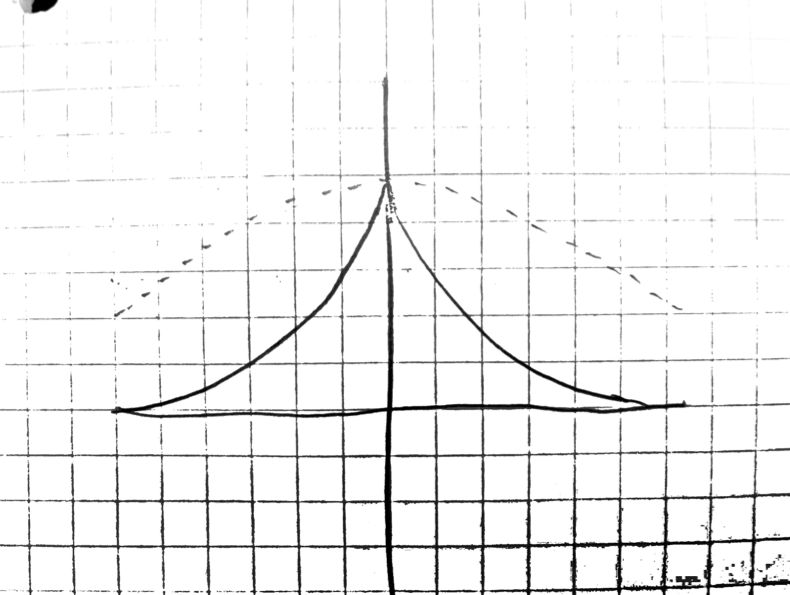
\includegraphics[width=\linewidth]{small_a.png}
		\caption{Small a}
	\end{subfigure}
	\begin{subfigure}[b]{0.4\linewidth}
		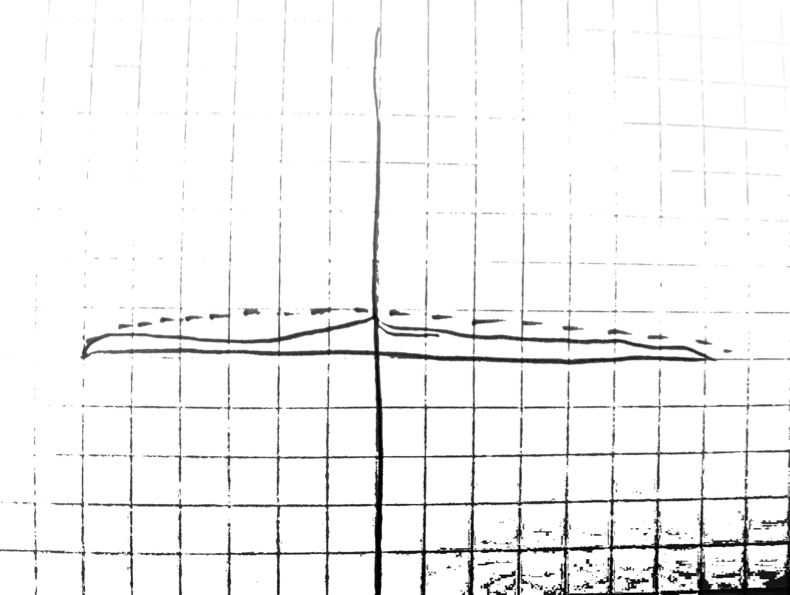
\includegraphics[width=\linewidth]{large_a.png}
		\caption{Large a}
	\end{subfigure}
\end{figure}
The spread of the wave functions has their amplitudes based on $a$, and they both have a symmetrical spread. 
\color{black}

\end{enumerate}

\item \textbf{The Quantum LC Circuit}

The quantum LC circuit forms the basis of the model of a superconducting flux qubit, as shown to the right. Fortunately, we can find the stationary state wave functions and energies of this system without explicitly solving the Schrodinger equation; instead, we will use the fact that the mathematical form of the Schrodinger equation of the quantum LC circuit is identical to that of the quantum harmonic oscillator to find the solutions. There is also a formal procedure for quantizing a classical system, called \textit{canonical quantization}.

\begin{enumerate}[a)]

\item The total energy of the classical harmonic oscillator yields the Hamiltonian of the quantum mechanical system, as shown below:
$$E_{QHO} = \frac{p^{2}}{2m} + \frac{1}{2}m\omega^{2}x^{2} \Rightarrow \hat{H}_{QHO} = \frac{p^{2}}{2m} + \frac{1}{2}m\omega^{2}x^{2}$$
where $\omega = \sqrt{k/m}$. We can derive the Hamiltonian of the quantum LC circuit via a similar analogy.

The total energy of the classical LC circuit is the sum of the electrical energy stored in the capacitor $E_{C}$ and the magnetic energy stored in the inductor $E_{L}$. Write down the total energy of the classical LC circuit in terms of electric charge ($q$), capacitance ($C$), magnetic flux ($\phi$), and inductance ($L$), then use that to write the Hamiltonian of the quantum LC circuit in terms of the operators $q$ and $\hat{\phi}$. 

\color{violet}
The total energy of a classical LC circuit is $E = E_{c} + E_{L} = \frac{1}{2}\frac{Q^{2}}{C} + \frac{1}{2}\frac{(N\Phi)^{2}}{L}$. In terms of the quantum circuit, it becomes $\frac{1}{2}\frac{q^{2}}{C} + \frac{1}{2}\frac{N\hat{\phi}^{2}}{L}$. 
\color{black}

\item We will now assert that the magnetic flux of the quantum LC circuit plays the same role as the momentum of the quantum harmonic oscillator, and that the electric charge plays the same role as the position, such that:
$$\hat{p} \Rightarrow \hat{\phi} \text{ and } \hat{x} \Rightarrow \hat{q}$$
By equating the kinetic energy term of the quantum harmonic oscillator with the magnetic energy
term of the quantum LC circuit, write down an expression for $m$ in terms of $L$. 

Then, by equating the potential energy term with the electrical energy term, write down an expression for $\omega$ in terms of $L$ and $C$. How does $\omega$ for the quantum LC circuit relate to the resonant frequency of the classical LC circuit?

\color{violet}
By equating $\frac{\hat{q}^{2}}{2m}$ and $\frac{(N\Phi)^{2}}{2L}$, the following expression will be made
$$m = \frac{L}{N^{2}}$$
And then, $\frac{1}{2}m\omega^{2}x^{2}$ and $\frac{1}{2}\frac{\hat{x}^{2}}{C}$.
$$\omega = \frac{N}{\sqrt{LC}}$$
\color{black}

\item Next, we’ll define a correspondence between the form of the operators of the quantum harmonic oscillator and quantum LC circuit, such that
\begin{gather*}
\hat{p} = -i\hbar\frac{d}{dx} \Rightarrow \hat{\phi} = -i\hbar\frac{d}{dq} \\
\hat{x} = x \Rightarrow \hat{q} = q
\end{gather*}
By using the substitutions above, write the time-independent Schrodinger equation for the quantum LC circuit in terms of $q$ and $\frac{d}{dq}$. \textit{Hint: the wave function is now a function of q, not x.}

\color{violet}
The time independent Schrödinger equation terms of position and momentum is $\left( -\frac{\hbar^{2}}{2m}\frac{\partial^{2}}{\partial x^{2}} + V(x) \right)\Psi(x) = E\Psi(x)$. By using the given substitutions, the following would be the new form of the Schrödinger equation
\begin{gather*}
E\Psi(q) = \left( -\frac{\hbar^{2}}{2m} \frac{\partial^{2}}{\partial q^{2}} + V(q) \right)\Psi(q)
\end{gather*}
\color{black}

\item By analogy with the quantum harmonic oscillator, write down the ground state wave function of the quantum LC circuit $\psi_{0}^{QLC} (q)$ in terms of $\omega$, $L$ and $q$, and sketch $|\psi_{0}^{QLC}(q)|^{2}$ vs. $q$. How do you interpret $|\psi_{0}^{QLC}(q)|^{2}$ in terms of measurements on the wave function?

\color{violet}
The ground state wave function $\psi_{0}(x)$ is $\left( \frac{m\omega}{\pi\hbar} \right)^{\frac{1}{4}}e^{-\frac{m\omega x^{2}}{2\hbar}}$. In terms of $\omega$, $L$, and $q$, the ground state wave function would be the following
\begin{gather*}
\psi_{0}^{QLC}(q) = \left( \frac{L\omega}{\pi\hbar N^{2}} \right)^{\frac{1}{4}} e^{\frac{\omega Lx^{2}}{2\hbar N^{2}}}
\end{gather*}
$|\psi_{0}^{QLC}(q)|^{2}$ would be the normalized wave function of the LC circuit, or the probability of measurement based on charge. 
\color{black}

\item What are the energies of the quantum LC circuit in terms of $\omega$? What are the energies in terms of $L$ and $C$?

\color{violet}
Since the LC circuit is proportional to a quantum harmonic oscillator, it has energies $\left(n + \frac{1}{2}\right)\hbar\omega$. In terms of $L$ and $C$, the energies are $\left(n + \frac{1}{2}\right)\hbar\frac{N}{\sqrt{LC}}$. 
\color{black}

\item Continuing our method of correspondences between the quantum harmonic oscillator and quantum LC circuit, we can write the electric charge and magnetic flux operators in terms of creation and annihilation operators:
$$\hat{q} = \sqrt{\frac{\hbar}{2L\omega}}(\hat{a}_{+} + \hat{a}_{-}) \text{ and } \hat{\phi} = i\sqrt{\frac{\hbar L\omega}{2}}(\hat{a}_{+} - \hat{a}_{-})$$
For the ground state, calculate the expectation value of the current through the inductor $\braket{I} = \frac{\braket{\phi}}{L}$ and the voltage across the capacitor $\braket{V} = \frac{\braket{q}}{C}$. What does this tell us about the average of measurements on the inductor current and capacitor charge for the ground state of the quantum LC circuit?

\color{violet}
The expectation value of $\braket{\phi}$ and $\braket{q}$ are the following
\begin{gather*}
\braket{\phi} = \int_{-\infty}^{\infty} \psi(q)^{*} \hat{\phi} \psi(q) dq = i\sqrt{\frac{\hbar L\omega}{2}} \int_{-\infty}^{\infty} \psi_{0}(q) (\hat{a}_{+} - \hat{a}_{-}) \psi_{0}(q) dq = i\sqrt{\frac{\hbar L\omega}{2}} \int_{-\infty}^{\infty} \psi_{0}(q) (\psi_{1}(q) - 0) dq \\
= i\sqrt{\frac{\hbar L\omega}{2}} \int_{-\infty}^{\infty} \psi_{0}(q)\psi_{q}(q) dq = 0\\
\braket{q} = \int_{-\infty}^{\infty} \psi(q)^{*} \hat{q} \psi(q)dq =  \sqrt{\frac{\hbar}{2L\omega}} \int_{-\infty}^{\infty} \psi_{0}(q) (\hat{a}_{+} + \hat{a}_{-}) \psi_{0}(q) dq = \sqrt{\frac{\hbar}{2L\omega}} \int_{-\infty}^{\infty} \psi_{0}(q) (\psi_{1}(q) + 0) dq = 0
\end{gather*}
This tells us that the inductor current and capacitor charge for the ground state of the quantum LC circuit are both always going to be 0, hence the LC circuit is not "charged". 
\color{black}

\item Give an example of a state that would yield $\braket{I} \neq 0$ and $\braket{V} \neq 0$ for the quantum LC circuit. 

\color{violet}
Some mixed state where $\psi(q) \neq \psi_{i}(q) + \psi_{j}(q)$ would have a non-zero current and voltage, because pure states have symmetrical wavefunctions, so it'll average out at the origin. 
\color{black}

\end{enumerate}

\item \textbf{Applications of Commutors}

As we will see shortly, commutators play an important role in the theory of quantum mechanics. Below are some applications that we have already encountered, which are special cases of more general theoretical statements.

\begin{enumerate}[a)]

\item \textit{Ehrenfest Theorem}

According to the Ehrenfest theorem, the rate of change of the expectation value $\braket{Q}$ is determined by the expectation value of the commutator of the Hamiltonian of that system $\hat{H}$ with the operator $\hat{Q}$:
$$\frac{d}{dt}\braket{Q} = \frac{i}{\hbar}\left(\braket{[\hat{H}, \hat{Q}]}\right) + \left\langle \frac{\partial \hat{Q}}{\partial t} \right\rangle$$
where $\braket{\frac{\partial \hat{Q}}{dt}} = 0$ or all of the operators we have considered so far (you can ignore it for this problem). Additionally, it tells us that the expectation values of quantities in a quantum system act like their classical analogs (i.e. $\braket{x} \Leftrightarrow x(t)$, $\braket{p} \Leftrightarrow p(t)$, etc.)

\begin{enumerate}[i)]

\item For the free particle, the potential $V(x) = 0$, so the Hamiltonians is given by $\hat{H} = \frac{\hat{p}^{2}}{2m}$. Calculate $\frac{d\braket{x}}{dt}$ and $\frac{d\braket{p}}{dt}$ for the free particle. Do the resulting equations match what you would expect for a free particle in classical mechanics?

\color{violet}
Using the given generalized Ehrenfest theorem, $\frac{d\braket{x}}{dt}$ and $\frac{d\braket{{p}}}{dt}$ could be prepared and calculated in the following manners
\begin{gather*}
\frac{d}{dt}\braket{x} = \frac{i}{\hbar}\left( \braket{[\hat{H}, \hat{x}]} \right) + \left\langle \frac{\partial \hat{x}}{\partial t} \right\rangle = \frac{i}{\hbar} \left( \left\langle \left[\frac{\hat{p}^{2}}{2m}, \hat{x}\right] \right\rangle \right) = \frac{i}{\hbar} \frac{\hbar}{im} \braket{\hat{p}} = \frac{1}{m}\braket{\hat{p}} \\
\frac{d}{dt} \braket{p} = \frac{i}{\hbar} \left( \left\langle \left[ \frac{\hat{p}^{2}}{2m}, \hat{p} \right] \right\rangle \right) + \left\langle \frac{\partial \hat{p}}{\partial t} \right\rangle = 0
\end{gather*}
The results do match the expectation for a free particle, since $\frac{d}{dt} \braket{x}$ is $\braket{p}$ classically and $\frac{d}{dt}\braket{p}$ is $-\braket{V'(x)}$. 
\color{black}

\item For the Quantum LC Circuit, the Hamiltonian is given by $\hat{H} = \frac{\hat{\phi}^{2}}{2L} + \frac{\hat{q}^{2}}{2C}$, where $\hat{q} = q$ is the electric charge operator and $\hat{\phi} = -i\hbar\frac{d}{d\hat{q}}$ is the magnetic flux operator. Calculate $\frac{d\braket{q}}{dt}$ and $\frac{d\braket{\phi}}{dt}$ for the Quantum LC Circuit. Do the resulting equations match what you would expect from circuit theory and classical electromagnetism?

\color{violet}
For $\frac{d\braket{q}}{dt}$ and $\frac{d\braket{\phi}}{dt}$, the Ehrenfest theorem applied to them is $\frac{i}{\hbar} \left( \braket{[\hat{H}, \hat{q}]} \right) + \left\langle \frac{\partial \hat{q}}{\partial t} \right\rangle$ and $\frac{i}{\hbar} \left( \braket{[\hat{H}, \hat{\phi}]} \right) + \left\langle \frac{\partial \hat{\phi}}{dt} \right\rangle$, which evaluates to the following
\begin{gather*}
\frac{d}{dt} \braket{\hat{q}} = \frac{i}{\hbar} \left( \left\langle\left[ \frac{\hat{\phi}^{2}}{2L}, \hat{q} \right] + \left[ \frac{\hat{q}^{2}}{2C}, \hat{q} \right]\right\rangle\right) = \frac{i}{\hbar} \frac{\hbar}{i2L} \braket{\hat{\phi}} = \frac{1}{2L}\braket{\hat{\phi}} \\
\frac{d}{dt} \braket{\hat{\phi}} = \frac{i}{\hbar} \left( \left\langle\left[ \frac{\hat{\phi}^{2}}{2L}, \hat{\phi} \right] + \left[ \frac{\hat{q}^{2}}{2C}, \hat{\phi} \right]\right\rangle\right) = \frac{i}{\hbar} \frac{\hbar}{i} \left\langle \frac{\partial}{\partial q} E_{C} \right\rangle = \frac{1}{2C} \left\langle \frac{\partial}{\partial q} \hat{q}^{2} \right\rangle = \frac{\braket{\hat{q}}}{C}
\end{gather*}
Classically, charge and magnetic flux oscillate in a sinusoidal manner, where charge decreases magnetic flux would increase and vice versa. The resulting equations do match such behavior.
\color{black}

\end{enumerate}

\item \textit{Uncertainty Principle}

As we discussed already, in a quantum system, the product of the spread in position measurements $x$ and momentum measurements $p$ has a lower limit of $\sigma_{x}\sigma_{p} \geq \frac{\hbar}{2}$. We interpret this as not being able to know the position and momentum of the particle simultaneously. Using commutators, we can express this relation in a more general form:
$$\sigma_{A}^{2}\sigma_{B}^{2} \geq \left( \frac{1}{2i} \braket{[\hat{A}, \hat{B}]} \right)^{2}$$
where $\hat{A}$ and $\hat{B}$ are operators that refer to measurablle quantities. 

\begin{enumerate}[i)]

\item Using the expression above, show that for position $x$ and momentum $p$, $\sigma_{x}\sigma_{p} \geq \frac{\hbar}{2}$.

\color{violet}
Given the above expression and the canonical commutation relation, the following is the uncertainty for $x$ and $p$
\begin{gather*}
\left( \frac{1}{2i} \left\langle  \left[ \hat{x}, \hat{p} \right] \right\rangle \right)^{2} = \left( \frac{1}{2i} \left\langle  \left[ \hat{x}, -i\hbar \frac{\partial}{\partial x} \right] \right\rangle \right)^{2} = \left( \frac{1}{2i} i\hbar \right)^{2} = \left( \frac{\hbar}{2} \right)^{2} \longrightarrow \sigma_{x}\sigma_{p} \geq \frac{\hbar}{2}
\end{gather*}
\color{black}

\item Using the expression above, show that for electric charge $q$ and magnetic flux $\phi$, $\sigma_{q}\sigma_{\phi} \geq \frac{\hbar}{2}$. What consequence does this have for being able to measure the charge on the capacitor and the magnetic flux in the inductor simultaneously in the Quantum LC Circuit?

\color{violet}
Same idea as the canonical operators, since the relations between the two are the same
\begin{gather*}
\left( \frac{1}{2i} \braket{[\hat{q}, \hat{\phi}]} \right)^{2} = \left( \frac{1}{2i} \left\langle \hat{q}, -i\hbar\frac{\partial}{\partial q} \right\rangle \right)^{2} = \left( \frac{
1}{2i} i\hbar \right)^{2} = \left( \frac{\hbar}{2} \right)^{2} \longrightarrow \sigma_{q}\sigma_{\phi} \geq \frac{\hbar}{2}
\end{gather*}
The consequence of this uncertainty on a quantum LC circuit is that the charge and magnetic flux, stored in separate components, cannot be measured accurately simultaneously. 
\color{black}

\end{enumerate}

\end{enumerate}

\end{enumerate}

\end{document}